\documentclass[letterpaper,12pt]{article}
\usepackage{tabularx} % extra features for tabular environment
\usepackage{amsmath}  % improve math presentation
\usepackage{graphicx} % takes care of graphic including machinery
\usepackage[margin=1in,letterpaper]{geometry} % decreases margins
\usepackage{cite} % takes care of citations
\usepackage[final]{hyperref} % adds hyper links inside the generated pdf file
\hypersetup{
	colorlinks=true,       % false: boxed links; true: colored links
	linkcolor=blue,        % color of internal links
	citecolor=blue,        % color of links to bibliography
	filecolor=magenta,     % color of file links
	urlcolor=blue         
}
\usepackage{blindtext}
\usepackage{minted}

\usepackage{caption}
\usepackage{subcaption}
%++++++++++++++++++++++++++++++++++++++++


\begin{document}

\title{Homework: Frozen Lake}
\author{ELEN E6885: Introduction to Reinforcement Learning}
\date{}
\maketitle




\section{Introduction}

\subsection{Algorithms}
The pseudo code for Policy Iteration, Value Iteration, Q-learning and SARSA:
\begin{figure}[h!]
     \centering
     \begin{subfigure}[b]{0.475\textwidth}
         \centering
         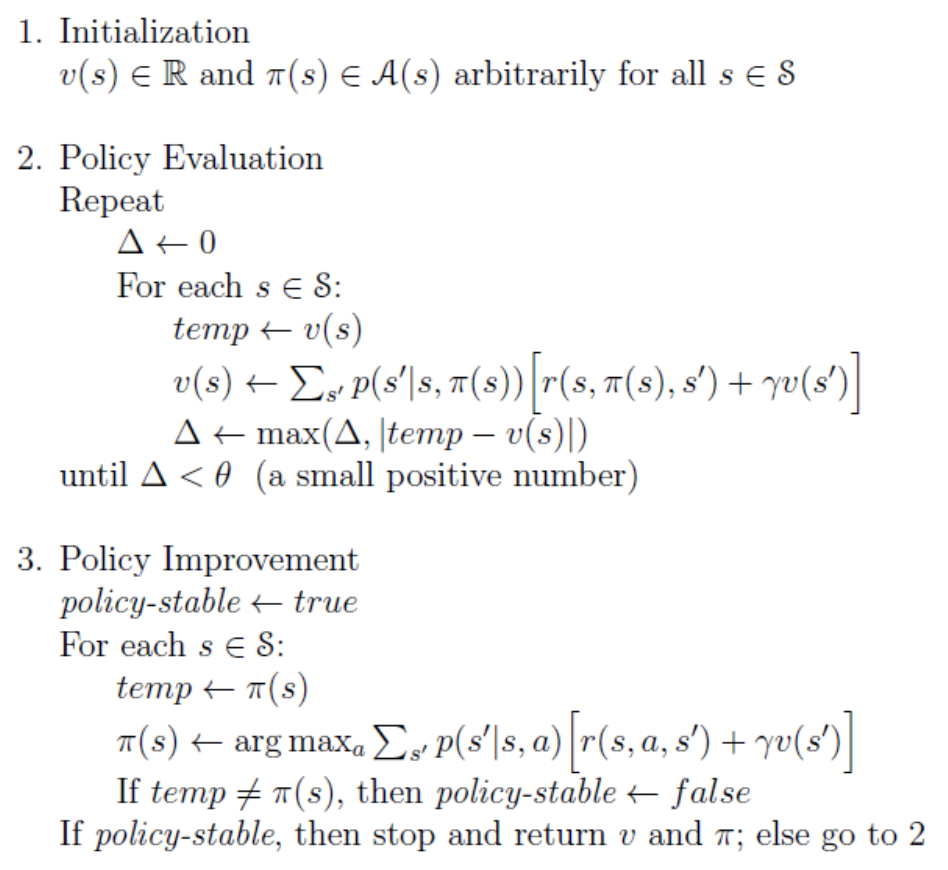
\includegraphics[width=\textwidth]{PI.png}
         \caption{Policy Iteration}
         \label{fig:1}
     \end{subfigure}
     \hfill
     \begin{subfigure}[b]{0.475\textwidth}
         \centering
         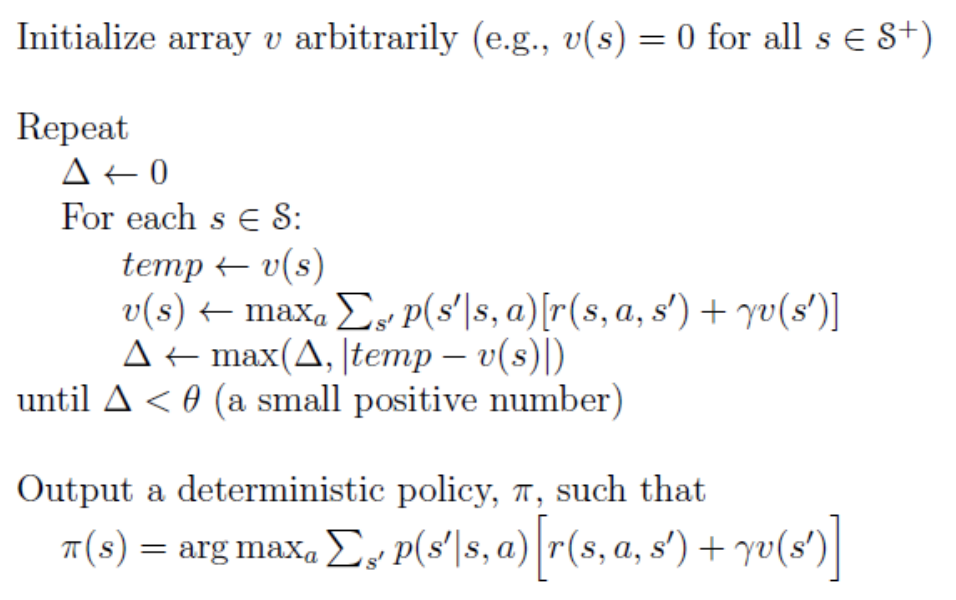
\includegraphics[width=\textwidth]{VI.png}
         \caption{Value Iteration}
         \label{fig:2}
     \end{subfigure}
     \vskip\baselineskip
     \begin{subfigure}[b]{0.475\textwidth}
         \centering
         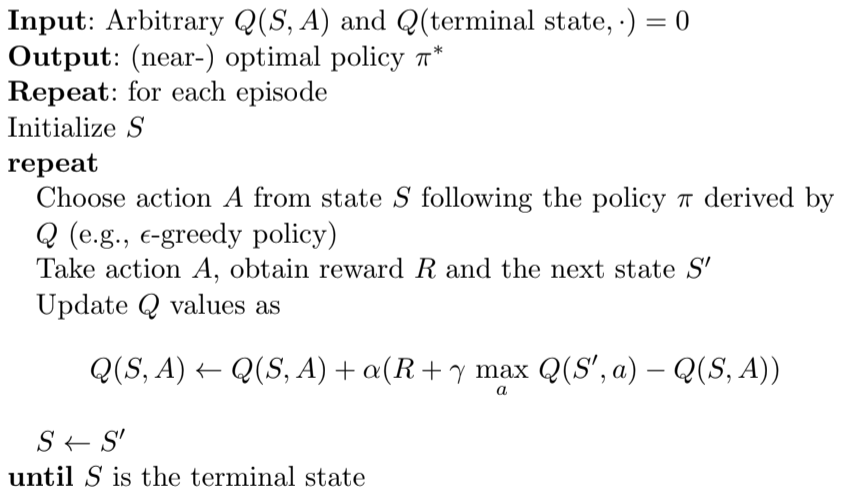
\includegraphics[width=\textwidth]{Q-learning.png}
         \caption{Q-Learning}
         \label{fig:3}
     \end{subfigure}
     \hfill
     \begin{subfigure}[b]{0.475\textwidth}
         \centering
         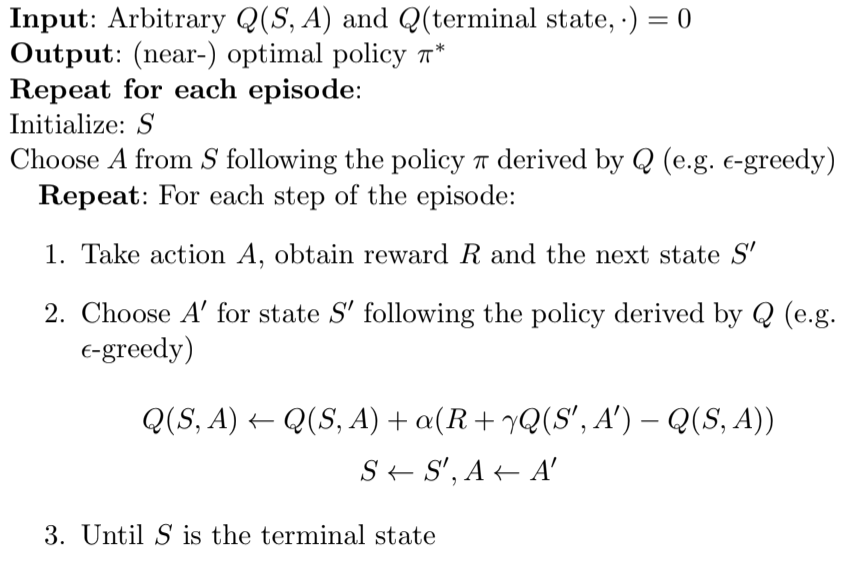
\includegraphics[width=\textwidth]{SARSA.png}
         \caption{SARSA}
         \label{fig:4}
     \end{subfigure}
        \label{fig:4 algorithms}
\end{figure}



\subsection{Implementation - OpenAI gym(FrozenLake-v1)}

\begin{itemize}
    \item Background \\
    Winter is here. You and your friends were tossing around a frisbee at the park when you made a wild throw that left the frisbee out in the middle of the lake. The water is mostly frozen, but there are a few holes where the ice has melted. If you step into one of those holes, you’ll fall into the freezing water. At this time, there’s an international frisbee shortage, so it’s absolutely imperative that you navigate across the lake and retrieve the disc. However, the ice is slippery, so you won’t always move in the direction you intend. The episode ends when you reach the goal or fall in a hole \cite{FrozenLake}.


    \item observation: \\
    The states form a 4 * 4 grid. There are 4 kinds of states. “S” is the safe starting point, “F” represents frozen surface, which is safe as well. “H” represents a hole. You “fall to your doom” if you enter “H” states. “G” is your goal where the frisbee is located. \\
    \begin{center}
        S F F F \\
        F H F H \\
        F F F H \\
        H F F G \\
    \end{center}

    \item Actions: \\
    Type: Discrete(4) \\
    At each step, you can take 4 actions: “LEFT”, “DOWN”, “RIGHT”, “UP” represented by indices 0 to 3 respectively. Your next state is then given by the environment.
    
    \item Reward: \\
    You receive a reward of 1 if you reach the goal, and 0 otherwise.
    
    \item Episode Termination: \\
    The episode ends when you reach the goal or fall in a hole. 
\end{itemize}



\section{Environment Setup}
We are using Google Colab \cite{colab} to execute the code. Colaboratory, or “Colab” for short, is a product from Google Research, allowing anybody to write and execute arbitrary python code through the browser, and is especially well suited to machine learning, data analysis and education. More technically, Colab is a hosted Jupyter notebook service that requires no setup to use, while providing free access to computing resources including GPUs. \\
\\
Steps to use the environment with start code: \\
1. Upload the start code onto your Google Drive Account and open the FrozenLake.ipynb by using colab. (Right click on the file -\textgreater open with -\textgreater Google Colaboratory) \\
2. Mount the Google Drive onto the Colab as the storage location \\
Following the instructions returned from the below cell. You will need to click a web link and select the google account you want to mount (The one that you upload the start code), then copy the authorication code to the blank, press enter.
\begin{minted}[frame = single]{python}
from google.colab import drive
drive.mount('/content/gdrive')
\end{minted}
3. Append the directory location where you upload the start code folder to the sys.path 
\begin{minted}[frame = single]{python}
import sys
sys.path.append('/content/gdrive/My Drive/<dir/to/start/code/folder>'))
\end{minted}
4. Then follow the detailed instructions step by step in FrozenLake.ipynb.



\section{Task} \label{sec:task}
You need to implement the following algorithms in RLalgs folder: Epsilon-Greedy, Policy Iteration, Value Iteration, Q-Learning and SARSA. Follow the detailed instructions step
by step in FrozenLake.ipynb which interactively show the result of each algorithms. We also have gym-tutorial.ipynb for you to get familiar with Gym package.

\section{Submission Instructions} \label{sec:submission}
Please submit the following two files: \\
1. A pdf report (printed out from Jupiter notebook with all codes and outcomes). \\
2. A zip file including folder "RLalgs", and your Jupyter notebook source file (for us to check your results).

\begin{thebibliography}{99}
\bibitem{FrozenLake} http://gym.openai.com/envs/FrozenLake-v0/
\bibitem{colab} https://colab.research.google.com/notebooks/intro.ipynb\#recent=true

\end{thebibliography}


\end{document}
